\documentclass[runningheads]{llncs}
\usepackage{graphicx,amsmath,amssymb}
\usepackage{hyperref}
\usepackage{url}
\usepackage{cite}
\usepackage{subfig}
%\usepackage{algorithmic}
%\usepackage{algorithm}
\usepackage{multirow}
\usepackage[ruled, noline, algo2e, noend, linesnumbered]{algorithm2e}
\urlstyle{rm}

%\usepackage{fullpage}
%\renewcommand{\Pr}[2][]{\mathrm{Pr}_{#1} \left[\, #2 \, \right]}
\renewcommand{\Pr}[2][]{\mathrm{Pr}_{#1} [\, #2 \, ]}

%----------------------- Macros and Definitions --------------------------
%\setlength{\parindent}{0pt} % don't indent the beginning of a paragraph
%\setlength{\parskip}{1ex plus 0.5ex minus 0.5ex} % but put some (vert.) space between the paragraphs
\renewcommand{\baselinestretch}{0.95} 

\newcommand{\abs}[1]{\lvert#1\rvert}
\newcommand{\norm}[1]{\lVert#1\rVert}
\newcommand{\T}{\ensuremath{\mathcal{T}}}
\newcommand{\gen}{\ensuremath{\mathrm{gen}}}
\newcommand{\cross}{\ensuremath{\mathit{cross}}}
\newcommand{\pop}{\ensuremath{\mathrm{pop}}}
\newcommand{\cost}{\ensuremath{\mathit{cost}}}
\newcommand{\Lold}{\ensuremath{\mathcal{L}_\mathrm{old}}}
\newcommand{\Lcur}{\ensuremath{\mathcal{L}_\mathrm{cur}}}
\newcommand{\Lnew}{\ensuremath{\mathcal{L}_\mathrm{new}}}
\newcommand{\BigOh}{\ensuremath{\mathcal{O}}}
\newcommand{\ie}{i.e.\ }
\newcommand{\cf}{cf.\ }

\newcommand{\obacht}[2][nobody]{\marginpar{\raggedright \tiny \textbf{obacht:} #2 (#1)}}

% fix soda style qed
\let\oldendproof\endproof
\def\endproof{\hfill\ensuremath{\Box}\oldendproof}

\def\MPS{\textsc{MinPopScheduling}}
\def\Wlog{\mathop{\rm WLOG}\nolimits}

% Prevent inline formula breaking
%\relpenalty=99999
%\binoppenalty=99999

% set-up for algorithm2e
% \SetArgSty{}
% \setlength{\algomargin}{2.2ex}
% \SetInd{2ex}{0ex}
% \SetKw{Kwhr}{or}
% \SetKw{KwAnd}{and}
% \SetKw{KwRequire}{require:}
% \SetKw{KwInvariant}{invariant:}
% \SetKwRepeat{KwRepeat}{repeat}{until}
% \SetKwIF{If}{ElseIf}{Else}{if}{then}{else if}{else}{endif}
% \SetKwComment{Comment}{/* }{*/}
%\dontprintsemicolon

\begin{document}
\sloppy 
\title{A Mathematical Programming Approach to Marker-Assisted Gene Pyramiding\thanks{A preliminary version of this paper appeared in Proceedings of
 the 11th Workshop on Algorithms in Bioinformatics, WABI 2011 \cite{DBLP:conf/wabi/CanzarE11}}}
\author{
    Stefan Canzar\inst{1,}\thanks{Joint first authorship.} \and Mohammed El-Kebir\inst{2,3,**}%$^{, *}$
}

\titlerunning{Marker-Assisted Gene Pyramiding}

\institute{Center for Computational Biology, McKusick-Nathans Institute of Genetic Medicine, Johns Hopkins University School of Medicine, Baltimore, Maryland 21205, USA
 \and Centrum Wiskunde \& Informatica, Life Sciences Group,
  Science Park 123, 1098~XG Amsterdam, the Netherlands \and Centre for Integrative Bioinformatics VU (IBIVU), VU University Amsterdam, De Boelelaan 1081A, 1081 HV Amsterdam, the Netherlands}

\hypersetup{%
  pdftitle={Marker-Assisted Gene Pyramiding},% titel
  pdfauthor={S. Canzar, M. El-Kebir},  % authors
  pdfborder={0 0 1},
  pdfcreator={}, pdfproducer={},
  citebordercolor={0 .667 0},          % dark green
  linkbordercolor={.5812 .0665 .0659}, % Indian red
  urlbordercolor={0 0 .667}            % dark blue
}

\maketitle

\begin{abstract}
In the \emph{crossing schedule} optimization problem we are given an initial set 
of parental genotypes and a desired genotype, the ideotype. The task is to schedule
crossings of individuals such that the number of generations, the number of crossings,
and the required populations size are minimized. We present for the first time a 
mathematical model for the general problem variant and show that the problem is 
$\mathcal{NP}$-hard and even hard to approximate. On the positive side, we present
a mixed integer programming formulation that exploits the intrinsic combinatorial structure 
of the problem. We are able to solve a real-world instance to provable optimality in less
than $2$ seconds, which was not possible with earlier methods.

TODO:
\begin{itemize}
  \item Describe how to deal with multiple chromosomes. And drawback of assumption.
  \item Describe backbone constraints
  \item Heterozygous ideotype
\end{itemize}

%A \emph{genotype} consists of two bitstrings of size $m$. We are given a set of
%$n$ genotypes and a desired genotype called the \emph{ideotype}. By crossing
%two genotypes, new genotypes can be obtained. The probability of obtaining a
%particular genotype out of two genotypes can be computed in advance. This
%probability can be translated to a \emph{population size} in which, with a
%prescribed probability of success, the required genotype is present.
%
%In a \emph{crossing schedule} it is described which crossings are needed in
%order to obtain the ideotype. Every crossing schedule is assigned a cost; one
%parameter of the cost function is the total population size needed. We are
%interested in obtaining the minimum-cost crossing schedule.
%
%In this report, the problem is defined formally and an NP-hardness result is
%given. 
\end{abstract}

\section{Introduction}
Plant breeding is the practice of creating improved varieties of cultivated crops with for instance a higher yield, better appearance or enhanced disease resistance \cite{BC:2008}. Up to recently, selection of favorable traits has been solely on the basis of observable \emph{phenotype} \cite{Dekkers:2002}. With the availability of \emph{genetic maps}, containing the exact locations on the genome of genetic markers associated with desirable traits, selection at the \emph{genotypic} level has become possible \cite{Moose:2008}. This knowledge allows to design a schedule of crossings of individuals resulting ultimately in an individual with all alleles corresponding to desired favorable traits present. In the plant breeding literature this process is called \emph{marker-assisted gene-pyramiding} and the resulting plan a \emph{gene-pyramiding scheme} or a \emph{crossing schedule} \cite{Servin:2004,Collard:2008,Ye:2008}. In this work we consider a mathematical programming approach to the problem that asks to identify given (1) a genetic map, (2) an initial set of parental genotypes and (3) the desired genotype|the so called \emph{ideotype}|a crossing schedule that results most cost-efficiently in the ideotype with respect to the following three criteria. Firstly, it takes time for the progeny to mature such that a next crossing can be performed. So the \emph{number of generations} is a measure on the time it takes to execute the crossing schedule. Secondly, every crossing between two individual plants requires an effort from the breeder, e.g.\ plants have to be treated such that they flower at the same time. So typically the \emph{number of crossings} is also to be minimized. Thirdly, in order to obtain the genotypes required by the schedule, for every crossing a specific number of offspring need to be generated among which the desired genotype is expected to be present. Simply speaking, the more difficult it is to obtain the desired genotype out of its parental genotypes, the larger the required number of offspring will be. Since every individual in the offspring has to be screened for having the desired genotype, the \emph{total population size} is also to be minimized.

%\begin{figure}
%\center
%\subfloat[Without selfing, requires 4 generations, 5 crossings and a total population size of 816.]{
%\label{fig:crossingschedule-1} 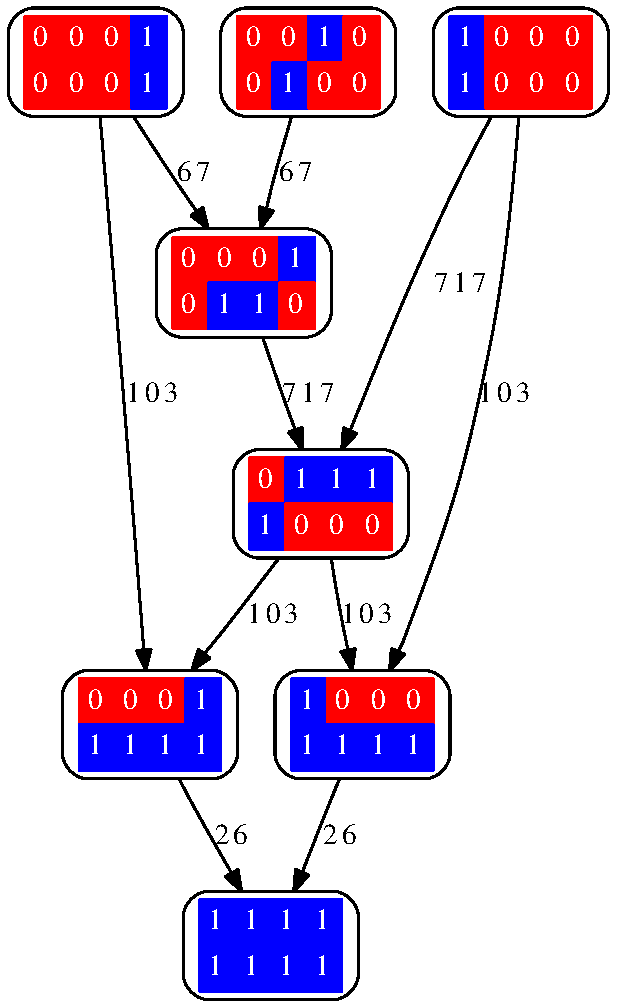
\includegraphics[scale=0.3]{images/schedule-1}
%}
%\hspace{1cm}
%\subfloat[With selfing, requires 3 generations, 3 crossings and a total population size of 3176.]{
%\label{fig:crossingschedule-2} 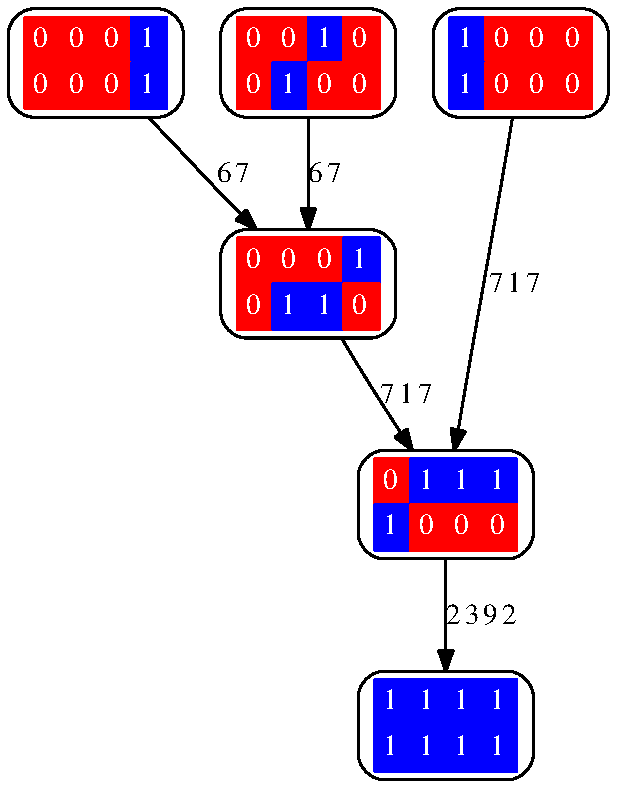
\includegraphics[scale=0.3]{images/schedule-2}
%}
%\caption{Example crossing schedules. The genotypes of the three parents are in the first generation, whereas the final generation contains the ideotype.}
%\label{fig:crossingschedule}
%\end{figure} 
%
%In Figure~\ref{fig:crossingschedule} two example crossing schedules are given. There we can see that a crossing schedule is a directed acyclic graph (DAG) whose source nodes correspond to the original parental genotypes and whose target node is the ideotype. Since every genotype is obtained from two parents (which need not be distinct), the in-degree of every inner node is exactly two.

\subsubsection{Related work.}
\label{sec:prev_work}
Most work on gene pyramiding lacks a formal framework; instead only an overview of guidelines and rules of thumb is given \cite{Ye:2008,Ishii-I:2007,Ishii-II:2007}. A notable exception, however, is the work by Servin et al.\ \cite{Servin:2004} who were the first to introduce a special case of the problem considered in this paper in a formal way. The authors show how to make use of the genetic map in determining the population sizes needed for all crossings. Contrary to our formulation, they allow a genotype to only participate in one crossing. In addition, very restrictive assumptions about the genotypes of the initial parents were made. These restrictions allowed the authors to exhaustively enumerate all crossing schedules and compare them in terms of population size needed. By introducing a heuristic, which partially alleviates the restriction on re-use of genotypes, the authors could compute smaller population sizes for the instances considered.
%It is unfortunate that Servin's work has passed relatively unnoticed by the plant breeding community. 
Later papers by Ishii and Yonezawa \cite{Ishii-I:2007,Ishii-II:2007} assume that target genes are always unlinked, which imposes a lower bound on the genetic distance of pairs of target genes. Similar to our work, in \cite{Ishii-I:2007,Ishii-II:2007} the number of generations, number of crossings and the total population size are identified as important attributes. An experimental evaluation is performed on manually obtained crossing schedules having different topologies for a fixed number of parents.
%Servin's and Ishii's work have in common that two stages are distinguished.
%First they aim to obtain a heterozygous genotype containing all target alleles.
%After which, using this genotype the ideotype is obtained. Ishii and Yonezawa
%describe this latter stage in a separate paper \cite{Ishii-II:2007}.

\subsubsection{Our contribution.}

In this work we lift the restrictions imposed by Servin et al.\ and consider a more general variant of the problem where genotypes are allowed to be re-used and no assumption about the initial parental genotypes is made. For the first time we formulate a mathematical model of the general problem. We show NP-hardness using an approximation-factor preserving reduction from an inapproximability result follows. We introduce a mixed integer linear program (MIP) formulation which exploits various aspects of the inherent combinatorial structure of the problem and
which approximates the non-linear objective by a piecewise linear curve.
Finally, we show that our approach is capable of solving real-world instances to provable optimality within a precise mathematical model, which was not possible
with earlier methods.


The rest of the paper is organized as follows. We start by formally defining the problem. In Section~\ref{sec:complexity} we show hardness of the problem.
In Section~\ref{sec:method} we introduce our method and state a MIP formulation for the problem. A thorough experimental evaluation
of our algorithm on a real-word instance and on randomly generated instances is presented in Section~\ref{sec:exp}. We conclude with a discussion on our results in Section~\ref{sec:discussion}.
%We conclude by considering a real-word instance and showing how our method fares against the heuristic given by Servin. \obacht[mohammed]{Say something about generated instances. And say something like: The contribution of this paper is twofold: firstly we continue on the work of Servin and for the first time give a complete mathematical abstraction of the concepts playing a role in marker-assisted gene pyramiding, secondly we give a method that results...}


\section{Problem definition}

A \emph{genotype} $C$ is a $2 \times m$ matrix whose elements are called \emph{alleles}. The two rows, $C_{1,\cdot}$ and $C_{2,\cdot}$, are called the lower and upper \emph{chromosome}, respectively. Each column in $C$ corresponds to a \emph{locus}. So at a locus $p$ two alleles are present, which we denote by $c_{1,p}$ and $c_{2,p}$. A locus is said to be \emph{homozygous} if its two alleles are identical, otherwise it is \emph{heterozygous}. Likewise, a genotype is homozygous if all its loci are homozygous, otherwise the genotype is said to be heterozygous. The desired genotype is called the \emph{ideotype}, which we denote by $C^*$. In plant breeding often pure lines are desired, as they allow for instance for the production of F1 hybrids \cite{BC:2008}. Therefore for the remainder of the paper we assume the ideotype to be homozygous. In this case, actual alleles can be classified as being present in the ideotype or not. Hence, the alleles in any genotype $C$ are binary.

We represent a \emph{crossing schedule} as a \emph{connected directed acyclic graph} (DAG) whose nodes are labeled by genotypes. Specifically, the source nodes correspond to the initial parental genotypes. A non-source node, which we refer to as an \emph{inner node}, corresponds to a crossing. The single target node is labeled by the ideotype. The arcs are directed towards the ideotype and relate a parent with its child. Since a genotype is obtained from two parents, the in-degree of an inner node is exactly 2. The two parents of a node need not be distinct. We say that a genotype is obtained via \emph{selfing} if its two parents are identical. From the topology of a crossing schedule the number of generations and the number of crossings can be inferred. The number of generations is the length of the longest path from a source node to the target node. On the other hand, the number of crossings corresponds to the number of inner nodes. In Figure~\ref{fig:pepper} an example crossing schedule is given.

%\begin{figure}
%\center
%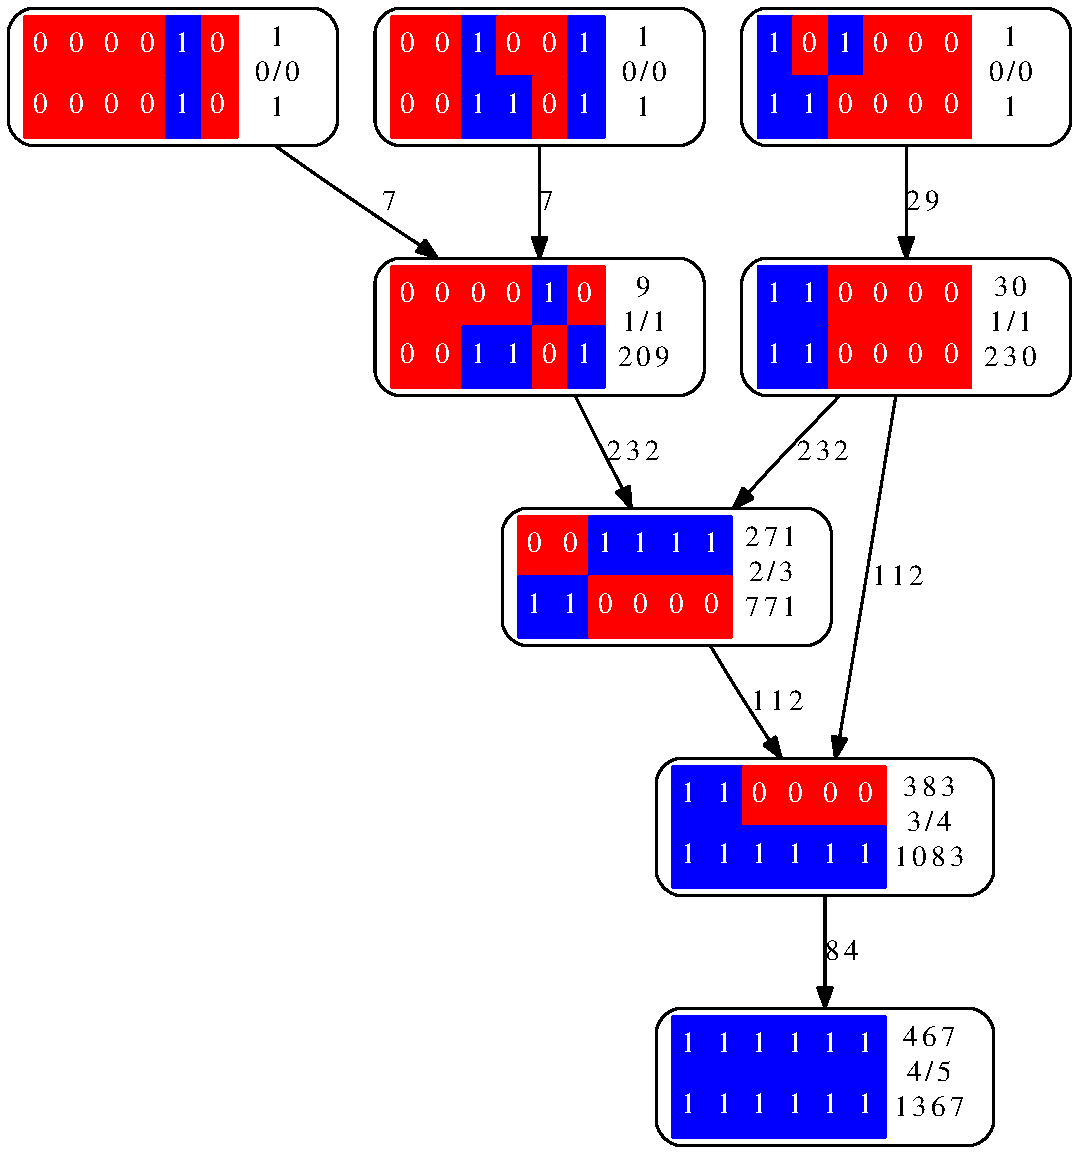
\includegraphics[scale=0.45]{images/example-schedule}
%\caption{Example crossing schedule, where $\cost(I) = 100 \cdot \gen(I) + 100
%\cdot \cross(I) + \pop(I)$. Per node $I$, from top to bottom and left to right:
%$\pop(I)$, $\gen(I)$, $\cross(I)$ and $\cost(I)$.}
%\label{fig:example-schedule}
%\end{figure}

The third attribute of a crossing schedule, the \emph{total population size}, is the sum of the population sizes implied by the crossings represented by inner nodes. Let $C$ be the genotype of an inner node and let $D$ and $E$ be the genotypes of the two parents of $C$. Later, we will show what the probability $\Pr{D,E \rightarrow C}$ of obtaining $C$ out of $D$ and $E$ is. For now we denote this probability with $\rho$. The population size $N(\rho, \gamma)$ corresponding to $\rho$ is the number of offspring one needs to generate in order to find with a given \emph{probability of success} $\gamma$ an individual with genotype $C$ among the offspring. Since $\rho$ is the probability of success in a Bernoulli trial, the probability that none of the $N(\rho, \gamma)$ offspring have genotype $C$ is $(1 - \rho)^{N(\rho,\gamma)} = 1-\gamma$. Therefore we have that
\begin{equation}
\label{eq:popsize}
N(\rho, \gamma) = \frac{\log(1-\gamma)}{\log(1-\rho)}.
\end{equation}
As also remarked in \cite{Servin:2004}, it is sensible to have an upper bound on every population size in the schedule, as depending on the plant species only a limited number of offspring can be generated. For that purpose we define $N_\mathrm{max}$ to be the \emph{maximal population size} to which every crossing in a crossing schedule has to adhere.

In diploid organisms, the genotype of a zygote is obtained by the fusion of two haploid gametes originating from one parent each. So one of the chromosomes of the resulting genotype $C$, say $C_{1,\cdot}$, corresponds to a gamete given rise to by $D$ and the other chromosome corresponds to a gamete produced by $E$. A gamete is the result of a biological process called \emph{meiosis} where in pairs of homologous chromosomes crossover events may occur. In our setting, this means that an allele $c_{1,p}$ corresponds to either $d_{1,p}$ or $d_{2,p}$ (where $1 \leq p \leq m$). In case a pair of alleles at loci $p$ and $q$ of $C_{1,\cdot}$ do not correspond to the same chromosome of $D$, we say that a \emph{crossover} has occurred between loci $p$ and $q$ (see Figure~\ref{fig:pepper}). From the genetic map, the probability of having a crossover between any pair of loci can be inferred using for instance Haldane's mapping function \cite{Haldane:1919}.
%By definition a crossover probability is at most $0.5$.
Let $R$ be a $m \times m$ matrix containing all crossover probabilities. Due to the nature of meiosis, we have that $r_{p,q} \leq 0.5$ for $1 \leq p < q \leq m$. Let $s = (\nu(1),\dots,\nu(k))$ be an ordered sequence of heterozygous loci in $D$. The probability of obtaining $C_{1,\cdot}$ out of $D$, i.e.\ $\Pr{D \rightarrow C_{1,\cdot}}$, is then as follows \cite{Servin:2004}. If there is an allele in $C_{1,\cdot}$ that does not occur in $D$ at the same locus then $\Pr{D \rightarrow C_{1,\cdot}} = 0$. Otherwise, if $s$ is empty then $\Pr{D \rightarrow C_{1,\cdot}} = 1$. Otherwise
\begin{equation}
\label{eq:single_prob}
\Pr{D \rightarrow C_{1,\cdot}} = \frac{1}{2} \prod_{i=1}^{k-1}
\begin{cases}
r_{\nu(i),\nu(i+1)} & \hspace{-.2cm}\mbox{\scriptsize if $c_{1, \nu(i)} = d_{1, \nu(i)} \wedge c_{1, \nu(i+1)} = d_{2, \nu(i + 1)}$}\\
                     & \hspace{-.2cm}\mbox{\scriptsize or $c_{1, \nu(i)} = d_{2, \nu(i)} \wedge c_{1, \nu(i+1)} = d_{1, \nu(i + 1)}$}\\
1 - r_{\nu(i),\nu(i+1)} & \hspace{-.2cm}\mbox{\scriptsize otherwise.}
\end{cases}
\end{equation}
We can now compute $\Pr{D,E \rightarrow C}$ using the following lemma.
\begin{lemma}
\label{lem:probability}
The probability of obtaining $C$ out of genotypes $D$ and $E$ is
\begin{equation}
\label{eq:combined_prob}
\Pr{D, E \rightarrow C} =
\begin{cases}
  \, \Pr{D \rightarrow C_{1,\cdot}} \cdot \Pr{E \rightarrow C_{2,\cdot}} & \mbox{if $C_{1,\cdot} = C_{2,\cdot}$}\\
  \begin{aligned}
    &  \Pr{D \rightarrow C_{1,\cdot}} \cdot \Pr{E \rightarrow C_{2,\cdot}}\\
    &  \quad \quad + \Pr{E \rightarrow C_{1,\cdot}} \cdot \Pr{D \rightarrow C_{2,\cdot}}
  \end{aligned} & \mbox{if $C_{1,\cdot} \neq C_{2,\cdot}$}\\
\end{cases}
\end{equation}
\end{lemma}

\begin{proof}
It holds that either $C_{1,\cdot}$ is obtained from $D$ and $C_{2,\cdot}$ is obtained from $E$,
or vice versa. Thus, we have
\begin{equation*}
\Pr{D, E \rightarrow C} = \Pr{((D \rightarrow C_{1,\cdot}) \cap (E \rightarrow C_{2,\cdot})) \cup ((E \rightarrow C_{1,\cdot}) \cap (D \rightarrow C_{2,\cdot}))}.
\end{equation*}
Due to independence, it holds that
\begin{equation*}
\Pr{D \rightarrow C_{1,\cdot} \cap E \rightarrow C_{2,\cdot}} = \Pr{D \rightarrow C_{1,\cdot}} \cdot \Pr{E \rightarrow C_{2,\cdot}},
\end{equation*}
and
\begin{equation*}
\Pr{D \rightarrow C_{2,\cdot} \cap E \rightarrow C_{1,\cdot}} = \Pr{D \rightarrow C_{2,\cdot}} \cdot \Pr{E \rightarrow C_{1,\cdot}}.
\end{equation*}
Recall that %\cite{MR:2006}
\begin{equation*}
\Pr{A \cup B} = \Pr{A}+ \Pr{B} - \Pr{A \cap B}.
\end{equation*}
Let $A = (D \rightarrow C_{1,\cdot}) \cap (E \rightarrow C_{2,\cdot})$ and $B = (E \rightarrow
C_{1,\cdot}) \cap (D \rightarrow C_{2,\cdot})$. If $C_{1,\cdot} \neq C_{2,\cdot}$ then $\Pr{A \cap B}$ is 0.
Otherwise, we have that $\Pr{A} = \Pr{B} = \Pr{A \cap B}$. 
\end{proof}

A common way to deal with multiple objectives is to consider a convex combination of the objective criteria involved \cite{Steuer:1986}. Given a crossing schedule, let $\mathrm{crs}$, $\mathrm{gen}$ and $\mathrm{pop}$ denote the number of crossings, number of generations and the total population size, respectively. For $\lambda_\mathrm{crs},\lambda_\mathrm{gen},\lambda_\mathrm{pop} \geq 0$ and $\lambda_\mathrm{crs}+\lambda_\mathrm{gen}+\lambda_\mathrm{pop} = 1$, the \emph{cost} of that crossing schedule is given by the convex combination
%\begin{equation} \label{eq:cost}
$  \lambda_\mathrm{crs} \cdot \mathrm{crs} + \lambda_\mathrm{gen} \cdot \mathrm{gen} + \lambda_\mathrm{pop} \cdot \mathrm{pop} $.
%\end{equation}
%\vspace{-.5cm}
\begin{problem}[\textsc{CrossingSchedule}]
Given $\mathcal{P} = \{C^1,\ldots,C^n\}$, the set of parental genotypes we start with, the homozygous ideotype $C^* \not \in \mathcal{P}$, the recombination matrix $R$, the desired probability of success $\gamma \in (0,1)$, the maximal population size $N_\mathrm{max}\in \mathbb{N}$  allowed per crossing, and a vector $\lambda$ of the cost efficients, problem \textsc{CrossingSchedule} asks for a crossing schedule of minimum cost.% \eqref{eq:cost}.
\end{problem}

\section{Complexity of the problem}
\label{sec:complexity}

We show that the problem is NP-hard even for the case where we are only minimizing the number of crossings.
%, i.e.\ $\lambda_\mathrm{crs}=1$ and $\lambda_\mathrm{gen},\lambda_\mathrm{pop} = 0$. 
We do this by giving a polynomial-time reduction from the decision problem \textsc{SetCover}, which asks given a universe $U$ and a collection of subsets $\mathcal{S} \subseteq 2^U$ whether there exists a cover $\mathcal{C} \subseteq \mathcal{S}$ of cardinality at most $k$ whose union is $U$ \cite{Karp:1972}. Let $(U, \mathcal{S}, k)$, where $U = \{e_1, \ldots, e_n\}$ and $\mathcal{S} = \{S_1, \ldots, S_l\}$, be a problem instance of \textsc{SetCover}. The corresponding problem instance of \textsc{CrossingSchedule} is obtained by letting the loci correspond to the elements in $U$ and the initial set of parents to the subsets in $\mathcal{S}$. The first chromosome of a parent $C^i$ has a 1 at locus $p$ if $p \in S_i$. The second chromosomes of all parental genotypes consists of only zeros. The ideotype has 1 alleles at every locus. In the cost function we only consider the number of crossings, i.e.\ $\lambda_\mathrm{crs} = 1$ and $\lambda_\mathrm{gen} = \lambda_\mathrm{pop} = 0$. The reduction can be done in polynomial time (in fact in $\BigOh(nl)$ time). In order to show that the reduction works, we have to show that the following holds.
\begin{lemma}
\label{lem:NP-hardness}
There is a cover of cardinality at most $k$ if and only if the cost of the optimum schedule is at most $k$.
\end{lemma}
\begin{proof}
$(\Rightarrow)$ Let $\mathcal{C} \subseteq \mathcal{S}$ be a cover such that
$|\mathcal{C}| \leq k$. Recall that every subset $S \in \mathcal{S}$
corresponds to one parent. So with $|\mathcal{C}| - 1$ crossings we can obtain
an individual whose genotype contains at least one 1 at every locus. The
ideotype can then be obtained by a selfing step. The corresponding schedule $G$
contains thus $|\mathcal{C}|$ crossings. Therefore, the optimum schedule $G^*$
contains at most $|\mathcal{C}| \leq k$ crossings.

$(\Leftarrow)$ Let $G^*$ be the optimum crossing schedule, and let $m$ be the
number of crossings in $G^*$. We have that $m \leq k$. We claim that the final
crossing in $G^*$ is a selfing step. Assume for a contradiction that this is
not the case. Let $D$ and $E$ be the two distinct genotypes whose
crossing resulted in $C^*$. We either have $D \not \in \mathcal{P}$ or $E \not \in
\mathcal{P}$, as if both $C$ and $D$ were to be in $\mathcal{P}$ then they would be equal
(recall that the second chromosome of genotypes in $\mathcal{P}$ has only zeros). Now
assume that $E \not \in \mathcal{P}$. The genotype $C^*$ can also be obtained by
selfing $D$. Since $E \not \in \mathcal{P}$, we require a crossing to obtain $E$
from its parents. So by obtaining $C^*$ via a selfing of $D$, the number of
crossings is at least one less than originally the case. This contradicts our
assumption that $G^*$ is optimal. Hence, the final crossing in $G^*$ is a
selfing.

All other $m - 1$ crossings involve two distinct individuals (i.e.\ no
selfing); the argument for this is as follows. Suppose for a contradiction that
there is a non-final selfing step involving an individual $C$ in $G^*$. Because
the selfing is non-final, the resulting individual $C'$ participates in another
crossing. Instead of using $C'$ in this crossing, we could have used $C$ and
ended up with a schedule with fewer crossing than $G^*$. This would be a
contradiction however.

So now we have $m-1$ crossings, each involving two distinct individuals. Let
$G^\prime$ be the subgraph of $G^*$ that contains these crossings. We have that
$G^\prime$ is connected as $G^*$ was connected. We now want to bound the number
of parents in $G^\prime$. There can be at most $m$ parents in $G^\prime$, as
the largest number of crossings is achieved when we have a binary tree with
$m-1$ inner nodes rooted at the pre-final individual. Since parents
correspond to subsets in $\mathcal{S}$ and since crossing them together
resulted in the ideotype, we have that there is a cover of at most $m$ subsets.
As $m \leq k$, there is a cover of cardinality at most $k$.
\end{proof}
Note that the reduction preserves the approximation factor, as the number of crossings equals the number of subsets in the cover. There is an inapproximability result for \textsc{SetCover}: it cannot be approximated within $\BigOh(\log n)$ unless {P = NP} \cite{Raz:1997}. Because of the approximation factor preserving reduction, this also holds for \textsc{CrossingSchedule}. In sum, the following theorems hold.
\begin{theorem}
\textsc{CrossingSchedule} is NP-hard.
\end{theorem}

\begin{theorem}
  Approximating \textsc{CrossingSchedule} within $\BigOh(\log n)$ is NP-hard.
\end{theorem}

\section{Method}\label{sec:method}
After exploring the combinatorial structure of the problem, we present an algorithm in which iteratively an MIP is solved. Details on the MIP formulation are given in Section~\ref{sec:ilp}.

Since we are considering homozygous ideotypes, we can assume without loss of generality that $C^*$ has only 1-alleles and derive a lower bound based on the minimum set cover as follows.
 The universe corresponds to the loci, i.e.\ $U = \{1, \ldots, m\}$, and the subsets $\mathcal{S} = \{S_1, \ldots, S_n\}$ correspond to $\mathcal{P} = \{ C^1, \ldots, C^n \}$. 
We define $p \in S_i$ if either $c^i_{1,p}=1$ or $c^i_{2,p} = 1$ where $1 \leq i \leq n$ and $1 \leq p \leq m$. The following lemma now follows.
\begin{lemma}
\label{lem:lb_crs}
The cardinality of a minimum set cover is a lower bound on the number of crossings of any feasible crossing schedule.
\end{lemma}
\begin{proof}
Let $\mathcal{C} = \{S_1,\ldots,S_k\}$ be a minimal cover with cardinality $k$. Assume without loss of generality that $C^*$ contains only 1-alleles.
% We claim that $k$ is a lower bound on the number of crossings. 
The subsets $\{S_1, \ldots, S_k\}$ that comprise $\mathcal{C}$ each correspond to an initial parental genotype, say that they correspond to $\{C^1,\ldots,C^k\}$. To obtain a crossing schedule with exactly $k$ source nodes, we need at least $k-1$ inner nodes/crossings. Since $\mathcal{C}$ is a minimum cover and since the ideotype is not an initial parental genotype, we need at least one more crossing for obtaining $C^*$. 
\end{proof}
Computing the minimum set cover is NP-hard. However, since in our experiments the number of loci and parents are relatively small, we are able to obtain the lower bound by solving a corresponding ILP \cite{Wolsey:1998} in a fraction of a second.

%From the lower bound on the number of crossings, $\mathit{LB}_\mathrm{crs}$, the following lower bound on the number of generations immediately follows.
%\begin{corollary}
%A lower bound on the number of generations %$\mathit{LB}_\mathrm{gen}$ 
%is $\lceil \log_2(\mathit{LB}_\mathrm{crs}) \rceil$.
%\end{corollary}

We can derive a lower bound for the total population size when considering consecutive pairs of loci for which there is no genotype in $\mathcal{P}$ containing 1-alleles at the same chromosome at both loci.
Let $(p,p+1)$ be such a pair of loci (where $1 \leq p < m$). For the ideotype to be obtained, there must be a genotype $C$ in the crossing schedule that contains 1-alleles at loci $p$ and $p+1$ on the same 
chromosome, while this condition does not hold for its parents $D$ and $E$. Clearly, $\Pr{D,E \rightarrow C} \leq r_{p,p+1}$. Plugging this into \eqref{eq:popsize} yields a lower bound on the population size
for that crossing and hence for the total population size. A tighter lower bound can be obtained when considering \emph{all} pairs of consecutive loci for which there are no genotypes in $\mathcal{P}$ containing
1-alleles at the respective loci on the same chromosome.\obacht[mohammed]{Why go from tight to tighter?} Let $\mathcal{L}$ be the set of such pairs of loci. One can easily verify that
\begin{equation}
\mathit{LB}_\mathrm{pop} := \sum_{(p,p+1) \in \mathcal{L}} N(r_{p,p+1},\gamma)
\end{equation}
is a lower bound on the total population size, as (i) for every $(p,p+1) \in \mathcal{L}$, $r_{p,p+1}$ is an upper bound on the probability of joining the two 1-alleles at loci $p$ and $p+1$, and (ii) 
the following lemma holds: \obacht[mohammed]{clarification about why (ii) is needed}
\begin{lemma}
\label{lem:pop_magic}
Let $p, q \in [0,0.5]$. Then
\[
N(p,\gamma) + N(q,\gamma) \leq N(p q,\gamma)
\]
\end{lemma}
\begin{proof}
From \eqref{eq:popsize} we have
\[
\frac{\log(1-\gamma)}{\log(1-p)} + \frac{\log(1-\gamma)}{\log(1-q)} \leq \frac{\log(1-\gamma)}{\log(1-p q)}.
\]
Since $\log(1-\gamma) < 0$, multiplying by $1/\log(1-\gamma)$ yields
\[
\frac{1}{\log(1-p)} + \frac{1}{\log(1-q)} \geq \frac{1}{\log(1-p q)}.
\]
Without loss of generality we can assume that $p \geq q$ and therefore it suffices to show that
%\[
%\frac{1}{\log(1-p)} \geq \frac{1}{\log(1-q)}.
%\]
%Thus
\[
\frac{2}{\log(1-p)} \geq \frac{1}{\log(1-p q)},
\]
which amounts to
\[
p(p q^2 - 2 q + 1) \geq 0.
\]
In case $p = 0$ the lemma follows, otherwise we can divide by $p$ and use $p^3 \geq p q^2$ yielding
\[
p^3 + 1 \geq 2q
\]
which holds since $q \leq 0.5$ and $p \geq 0$. 
\end{proof}

Using \eqref{eq:combined_prob} one can show that there is an optimal crossing schedule where all homozygous genotypes are obtained via selfings. 
\begin{lemma}
\label{lem:selfing}
There is an optimal schedule in which the (inner) homozygous genotypes are obtained via selfings.
\end{lemma}
\begin{proof}
We prove this by contradiction. Let $C$ be a homozygous genotype obtained
optimally but not via a selfing. Let $D$ and $E$ be the two parents of $C$.
Since $C$ is homozygous, i.e.\ $C_{1,\cdot} = C_{2,\cdot}$, we have that $\Pr{D \rightarrow
C_{1,\cdot}} > 0$ and $\Pr{E \rightarrow C_{1,\cdot}} > 0$. In other words, both $D$ and $E$ can
give rise to $C_{1,\cdot}$.

Let's look at what happens when we self either $D$ or $E$. The number of
generations and the number of crossings would not change for the worse. 
We claim that if we self the genotype that has the highest probability of 
giving rise to $C_{1,\cdot}$, we get that the probability of obtaining $C$ is at most the probability of obtaining $C$ via a crossing of $D$ and $E$.
Since $C$ is homozygous, we have by Lemma~\ref{lem:probability} that
\[
\Pr{D,E \rightarrow C} = \Pr{D \rightarrow C_{1,\cdot}} \cdot \Pr{E \rightarrow C_{1,\cdot}}.
\]
We assume without loss of generality that $\Pr{E \rightarrow C_{1,\cdot}} \leq \Pr{D \rightarrow C_{1,\cdot}}$. Therefore we have
\[
\Pr{D,E \rightarrow C} \leq \Pr{D \rightarrow C_{1,\cdot}}^2.
\]
So the population size needed for obtaining $C$ by selfing $D$ is at most the
population size that we needed to obtain $C$ out of $D$ and $E$. 
\end{proof}


Finally, parental genotypes that contain a $1$-allele at a locus at which all other parental genotypes contain all $0$ have to be used by any feasible schedule. To reduce the search space explored by the MIP solver we fix these \emph{compulsory} parental genotypes to be contained in any solution.

We present a MIP formulation for the problem variant where the number of crossings and the number of generations is fixed to $F$, respectively $G$. The reason for this is to be able to introduce cuts that ensure monotonically better solutions. In order to solve a problem instance, we iteratively consider combinations of $(F,G)$ starting from $F = \mathit{LB}_\mathrm{crs}$ and $G = 1 + \lceil \log_2 F \rceil$. In addition we enforce that the objective value of any feasible solution must be better than the currently best one. We do this by computing an upper bound $\mathit{UB}_\mathrm{pop}$ on the total population size, based on the best objective value found so far and the current values of $(F,G)$ (see Algorithm~\ref{alg:overall}, line~\ref{alg:UB_pop}). If at some point, say $(F^\prime,G^\prime)$, $\mathit{LB}_\mathrm{pop} \geq \mathit{UB}_\mathrm{pop}$ then we know that none of the combinations of $F^{\prime\prime} \geq F^\prime$, $G^{\prime\prime} \geq G^\prime$ will lead to a better solution. Therefore if $G = 1 + \lceil \log_2 F \rceil$ and $\mathit{LB}_\mathrm{pop} \geq \mathit{UB}_\mathrm{pop}$, we have found the optimal solution (see Algorithm~\ref{alg:overall}, line~\ref{alg:opt}). To guarantee termination for the case where $\lambda_\mathrm{crs} = \lambda_\mathrm{gen} = 0$, we stop incrementing $F$ as soon as it reaches a pre-specified parameter $\mathit{UB}_\mathrm{crs}$. Similarly, $\mathit{UB}_\mathrm{gen}$ is a pre-specified parameter bounding $G$. In Algorithm~\ref{alg:overall} the pseudo code is given.

\begin{algorithm2e}[h!]
\caption{\textsc{OptCrossingSchedule}$(\mathit{UB}_\mathrm{crs},\mathit{UB}_\mathrm{gen})$}
\label{alg:overall}
\KwIn{
  %$\mathit{LB}_\mathrm{crs}$ and $\mathit{LB}_\mathrm{pop}$ are lower bounds on the number of crossings and the population size, 
  $\mathit{UB}_\mathrm{crs}$ and $\mathit{UB}_\mathrm{gen}$ are the maximum number of crossings and generations considered.}
$\mbox{OPT} \leftarrow \infty$\\
%$G_\mathrm{max} \leftarrow \infty$\\
\For {$F \leftarrow \mathit{LB}_\mathrm{crs}$ \KwTo $\mathit{UB}_\mathrm{crs}$}
{
  \For {$G \leftarrow 1 + \lceil \log_2 F \rceil$ \KwTo $\min(F, \mathit{UB}_\mathrm{gen})$}
  {
   $\mathit{UB}_\mathrm{pop} \leftarrow \frac{1}{\lambda_\mathrm{pop}}(\mbox{OPT}-F\cdot\lambda_{crs}-G\cdot\lambda_{gen})$\\
 \nllabel{alg:UB_pop}    \lIf {$\mathit{LB}_\mathrm{pop} < \mathit{UB}_\mathrm{pop}$}
    {
      $\mbox{OPT} \leftarrow \min(\mbox{OPT}, \mbox{MIP}(F,G,\mathit{UB}_\mathrm{pop}))$\\
    }
    \lElse
    {
      $\mathit{UB}_\mathrm{gen} \leftarrow G - 1$
    }
  }
  \lIf {$\mathit{UB}_\mathrm{gen} \leq 1 + \lceil \log_2 F \rceil$}
  {
    \Return OPT
  }
}
 \nllabel{alg:opt} \Return OPT\\
\end{algorithm2e}

\subsection{MIP formulation}
\label{sec:ilp}
Given an instance to \textsc{CrossingSchedule} with initial parental genotypes $\mathcal{P}=\{C^1,\dots,C^n\}$, a feasible solution with $G$ generations and $F$ crossings can be characterized by the following five conditions: (i) The topology of the schedule is represented by a directed acyclic graph with $n$ source nodes $s_1,\dots, s_n$, one target node $t$, and $F-1$ additional nodes, where every non-source node has in-degree two. Parallel arcs are allowed and represent selfings. (ii) The longest path from a source node to the target node has length $G$. (iii) The alleles of each non-source node are derived from either the upper or lower chromosome of the node's respective predecessors. (iv) The genotype of a source node $s_i$ is $C^i$, the genotype of $t$ is $C^*$. (v) The probability of obtaining the genotype of an inner node $v$ is at least $1 - (1 - \gamma)^\frac{1}{N_\mathrm{max}}$ such that its corresponding population size is at most $N_\mathrm{max}$.

In the following we show how these conditions can be formulated as linear constraints. Throughout our formulation, we let $L:=F+n$ be the total 
number of nodes. Dummies $1 \leq i,j \leq L$ correspond to genotypes, loci are indexed by $1 \leq p,q \leq m$ and chromosomes are referred to by $1 \leq k,l \leq 2L$. For brevity's sake, in the remainder of the paper we will omit the linearization of products of binary variables. Unless otherwise stated, we applied a standard transformation \cite{Bradley:1977}: for a product $x\cdot y$ of binary variables $x$ and $y$ we introduce a new binary variable $z$ and require $z\leq x$, $z\leq y$, and $z\geq x+y-1$.
Similarly, we omit the details of the implementation of absolute differences of binary variables.

\subsubsection{Feasibility constraints.}
\label{sec:feasibility}

The first set of constraints encodes the structure of the underlying directed acyclic graph $D=(V,A)$. We assume a numbering of the vertices
according to their topological order. In particular, arcs always go from vertices $j<i$ to a vertex $i$ for $i,j\in V$. Based on the node numbering, the lower and upper chromosomes of a node $i \in V$ are respectively $2i-1$ and $2i$. For convenience we introduce a mapping function $\delta(k)$ that returns the node a chromosome $k$ corresponds to.
Then binary variables $x_{k,i}\in\{0,1\}$, $2n < k \leq 2L$, $1 \leq i<\delta(k)$, denote whether chromosome $k$ originates from genotype $i$, that is, they indicate an arc $(i,\delta(k))$.
Since a chromosome originates from exactly one genotype, we have
\begin{align}
  \label{eq:ilp_x_1}
  \sum_{j=1}^{\delta(k)- 1} x_{k,j} = 1 && 2n < k \leq 2L
\end{align}

To add:
\begin{enumerate}
  \item Out degree of all inner nodes must at least 1
  \item Backbone stuff
\end{enumerate}

We capture the second condition by fixing a path of length $G$ using the $x$ variables and by restricting the depth of all remaining nodes, represented by additional
integer variables, to be at most $G-1$. Implementing this condition requires the assumed ordering on vertices to be extended. For the sake of a clear discussion, we omit the details.

To model the third condition, we introduce 
binary variables $a_{k,p}$, $1 \leq k \leq 2L$, $1 \leq p \leq m$, which indicate the allele at locus $p$ of chromosome $k$. 
%Note that for chromosomes $k$ corresponding to initial parental genotypes, $a_{k,p}$, $1 \leq p \leq m$, is a constant rather than a variable.
In addition to knowing from which genotype a chromosome originates, we also need to know from which of the two chromosomes of that 
parental genotype an allele comes. Therefore we define binary variable $y_{k,p}$, $2n < k \leq 2L$, $1 \leq p \leq m$, to be $1$ if the allele at locus $p$
of chromosome $k$ comes from the lower chromosome of its originating genotype;
conversely $y_{k,p}$ is $0$ if the allele originates from the upper chromosome.
Now we can relate alleles to originating chromosomes. We do this by introducing
binary variables $g_{k,p,l}$, for $2n < k \leq 2L$, $1 \leq p \leq m$, and $1 \leq l<2\delta(k)-1$.
We define $g_{k,p,l} = 1$ if and only if the allele at locus $p$ of chromosome
$k$ originates from chromosome $l$ and has value 1. This is established through constraints
\begin{align}
  \label{eq:ilp_g1}
  g_{k,p,2i} - a_{2i,p} \cdot x_{k,i} \cdot (1-y_{k,p}) & = 0 && 2n < k \leq 2L, 1 \leq p \leq m, i < \delta(k)\\
 \label{eq:ilp_g2}
  g_{k,p,2i-1}   - a_{2i-1,p} \cdot x_{k,i} \cdot y_{k,p} &= 0 && 2n < k \leq 2L, 1 \leq p \leq m, i < \delta(k)
\end{align}
Finally, an allele is $1$ if and only if it originates from exactly one $1$-allele:
\begin{align}
  \label{eq:ilp_g3}
   a_{k,p} - \sum_{i = 1}^{\delta(k) - 1} (g_{k,p,2i-1} + g_{k,p,2i}) = 0&& 2n < k \leq 2L, 1 \leq p \leq m
\end{align}
The fourth property can be ensured by simply forcing the variables representing the alleles of the parental genotypes, i.e.~the source nodes,
and the alleles of the desired ideotype, that is, the target node, to the actual value of the respective allele. Thus for the parental genotypes we have $a_{2i-1,p} = c^i_{1,p}$ and $a_{2i,p}  = c^i_{2,p}$ for $1 \leq i \leq n, 1 \leq p \leq m$
and for the ideotype $a_{2L-1,p} = a_{2L,p} = c^*_{1,p}$ for $1 \leq p \leq m$.
The last property is enforced implicitly by the objective function, which is described in the following. 

\subsubsection{Objective function.}

%An optimal solution to our MIP represents a crossing schedule with minimum total population size using $G$ generations and $F$ crossings.
The probability of a given genotype $i$ giving rise to a specific chromosome $k$ determines the 
required population size (see \eqref{eq:popsize}). This probability in turn depends on the exact set of
crossovers necessary to generate chromosome $k$ and on the sequence $s$ of heterozygous
loci (see \eqref{eq:single_prob}). We define binary variable $\tilde{a}_{i,p}=1$ if and only if locus $p$ of genotype $i$ is heterozygous: $\tilde{a}_{i,p} = |a_{2i-1,p} - a_{2i,p}|$ for $1 \leq i \leq L, 1 \leq p \leq m$.
Now a genotype $i$ is heterozygous, indicated by $h_i=1$, if at least one of its loci is heterozygous: $h_i \geq \tilde{a}_{i,p}$ for  $1 \leq i \leq L, 1 \leq p \leq m$.
It is ensured that $h_i=0$ whenever $\tilde{a}_{i,p}=0$, $\forall 1 \leq p \leq m$, as $h_i=1$ would increase the required population size.

Concerning the dependence on the set of crossovers, we let integer variables $z_{k,p,q}$ indicate whether the segment between locus $p$ and $q$ of chromosome $k$ results from a crossover event:
\begin{align}
  z_{k,p,q} & = \sum_{r=p+1}^q |y_{k,r} - y_{k,r-1}| && 2n < k \leq 2L,\, 2 \leq p < q \leq m
\end{align}
The distinction between the two different cases in \eqref{eq:single_prob} is based on crossover events
between two successive heterozygous loci, i.e.~$\nu(i)$ and $\nu(i+1)$. We capture the sequence $s$ of heterozygous
loci used in \eqref{eq:single_prob} by binary variables $b_{i,p,q}$, which indicate a
maximal block of homozygous loci between heterozygous loci $p$ and $q$, $1 \leq p<q \leq m$, in genotype $i$, $1 \leq i \leq L$:
\begin{align}
  b_{i,p,q} & = \tilde{a}_{i,p}\cdot\tilde{a}_{i,q}\cdot\prod_{r=p+1}^{q-1}(1-\tilde{a}_{i,r})  && 1 \leq i \leq L, 1 \leq p<q \leq m
\end{align}
%Then binary variable $\bar{z}_{k,p,q,j}$, $1 \leq k \leq 2L$, $1 \leq p<q \leq m$, and $j<\delta(k)$, denotes the existence of at least one crossover event in a maximal homozygous block between loci
%$p$ and $q$ of chromosome $k$'s originating genotype $j$:
%\begin{align}\label{eq:whatever}
%  \bar{z}_{k,p,q,j} & = b_{j,p,q}\cdot\sum_{r=p+1}^{q}z_{k,r,j}  && 2n < k \leq 2L, 1 \leq p<q \leq m, j < \delta(k)
%\end{align}
%To allow for a linearization of constraint \ref{eq:whatever} according to the scheme described in the beginning of Section \ref{sec:ilp} we have to ensure that at most one crossover occurs in each maximal
%homozygous block. We accomplish this through constraints
%\begin{align}
%  \sum_{r=p+1}^q z_{k,r,j} \leq 1+\sum_{r=p+1}^{q-1} \tilde{b}_{j,r} && 2n < k \leq 2L,\, 1 \leq p <q \leq m,\, j < \delta(k) 
%\end{align}
%Clearly, if loci $p+1$ up to $q-1$ form a homozygous block, $\sum_{k=p+1}^{q-1} \tilde{b}_{j,k}=0$ and thus a feasible solution contains at most one crossover. Furthermore,
%the number of homozygous blocks enclosed by loci $p$ and $q$ is at most  $\sum_{k=p+1}^{q-1} \tilde{b}_{j,k}+1$ and hence we do not cut off any feasible solution.
%%\prod_{1\leq p<q\leq m}
We are now able to formulate the probability given in \eqref{eq:single_prob} in terms of our new binary variables. For that, let $\xi_k^j$ denote
the event of obtaining a chromosome $k$ from a genotype $j$. %where we have replaced in the second inequality $b_{j,p,q}\cdot\sum_{r=p+1}^{q}z_{k,r,j}$ by $\bar{z}_{k,p,q,j}$ according to \eqref{eq:whatever}.
Using variables $h$, $b$, and $z$, we can express $\Pr[]{\xi_k^j}$ as follows.
Under the assumption that $x_{k,j}=1$,
\begin{equation*}
\begin{split}\Pr[]{\xi_k^j}=(1-\frac{h_j}{2})&\prod_{p=1}^{m-1}\prod_{q=p+1}^m \bigg( (1-b_{j,p,q}) \\
%& + b_{j,p,q}\cdot (r_{p.q}\cdot \sum_{r=p+1}^{q}z_{k,r,j}+(1-r_{p,q})\cdot (1-\sum_{r=p+1}^{q}z_{k,r,j}))   \bigg)  
& + b_{j,p,q}\cdot (r_{p,q}\cdot z_{k,p,q}+(1-r_{p,q})\cdot (1-z_{k,p,q}))   \bigg)
\end{split}
\end{equation*}
For a homozygous genotype $j$ all elements in the upper product evaluate to 1 as desired. In the heterozygous case, every maximal homozygous block
contributes $r_{p,q}$ if it contains at least one crossover (first case in \eqref{eq:single_prob}), and $(1-r_{p,q})$ otherwise (second case in \eqref{eq:single_prob}).

Now the idea is to develop an appropriate approximation of the nonlinear function $N(p,\gamma)$
defining the required population size so that integer linear programming
techniques can be utilized. More precisely, we reduce $N(p)$ to a separable form \cite{Steuer:1986} that depends only on a single decision variable 
and approximate it by a piecewise linear function.
Using the fact that $(1-r_{p,q})\geq r_{p,q}$, $\forall 1\leq p<q<m$, we
define $\Delta r_{p,q}:=(1-r_{p,q})-r_{p,q}$ and rewrite the probability of event $\xi_k^j$, again assuming $x_{k,j}=1$ as
\begin{equation*}
\begin{split}
\Pr[]{\xi_k^j}&=(1-\frac{h_j}{2})\prod_{p=1}^{m-1}\prod_{q=p+1}^m \left((1-b_{j,p,q}) + b_{j,p,q}\cdot (1-r_{p,q}-\Delta r_{p,q} z_{k,p,q})\right)\notag\\
&=\exp\bigg(h_j\cdot\ln(\frac{1}{2})+\sum_{p=1}^{m-1}\sum_{q=p+1}^m b_{j,p,q}\cdot \ln(1-r_{p,q}) \\
&\qquad\qquad + \sum_{p=1}^{m-1}\sum_{q=p+1}^m b_{j,p,q} \cdot z_{k,p,q}\cdot \ln(\frac{r_{p,q}}{1-r_{p,q}}) \bigg)
\end{split}
\end{equation*}


Finally, if $j_1$ and $j_2$ are the two parental genotypes of chromosomes $k_1$ and $k_2$ forming genotype $i$, we compute in variable $\bar{z}_i$ the $\log$ probability of event $\xi^{j_1}_{k_1}\cap\xi^{j_2}_{k_2}$
as $\ln(\Pr[]{\xi^{j_1}_{k_1}})+\ln(\Pr[]{\xi^{j_2}_{k_2}})$. For that we have to sum over all possible $1 \leq j<i$ to identify $j_1$ and $j_2$:
\begin{equation}
 \label{eq:something}
 \begin{split}
 \bar{z}_i=\sum^{i-1}_{j=1}\sum_{l\in\{1,2\}}x_{k_l,j}\bigg(h_j\ln(\frac{1}{2})&+\sum_{p=1}^{m-1}\sum_{q=p+1}^m b_{j,p,q}\ln(1-r_{p,q})\\
 &+ \sum_{p=1}^{m-1}\sum_{q=p+1}^m  b_{j,p,q} \cdot z_{k_l,p,q} \ln(\frac{r_{p,q}}{1-r_{p,q}}) \bigg)   
 \end{split}
\end{equation}
\obacht{eq differs from conference version, see comment in .tex, MEK: it's good}

Notice that we neglect the possibility that the two chromosomes $k_1$ and $k_2$ may swap their originating genotypes as accounted for in the 
second case of equation \eqref{eq:combined_prob} and we therefore might underestimate the probability of success, respectively overestimate
the population size. We will discuss this simplification in Section \ref{sec:discussion}.

We develop an appropriate approximation of the nonlinear function $N(\rho, \gamma)$ defining the required population size so that integer linear 
programming techniques can be utilized.
More precisely, we are able to re-express the population size w.r.t.\ probability $p:=\Pr[]{j_1,j_2\rightarrow i}$ in separable form as: 
$$ N(p,\gamma) = \frac{\ln(1-\gamma)}{\ln(1-\mathrm e^{\bar{z}_i})} $$
We use $\ell$ segments to approximate the nonlinear function $N$ by a
piecewise-linear curve specified by the points $(d_j,N(d_j,\gamma))$ for
$j=1,\dots,\ell+1$. The idea of the \emph{$\lambda$-method} \cite{Steuer:1986} is to
express any point $p\in[d_1,d_{\ell+1}]$ as a convex combination of two adjacent
breakpoints $d_j$ and $d_{j+1}$, where  $p\in[d_j,d_{j+1}]$, and derive an
approximation for $N$ by weighing the function's values $N(d_j,\gamma)$ and
$N(d_{j+1},\gamma)$ accordingly. More precisely, we add for every $i$ the following
constraints (where $n < i \leq L$):
\begin{align}
  \sum_{j=1}^{\ell+1} \lambda^i_j &= 1&\\
  \sum_{j=1}^{\ell+1} \lambda^i_j\cdot d_j &= \bar{z}_i&\label{ttt}\\
  \lambda^i_j&\geq 0& j=1,\dots,\ell+1
\end{align}
Note that the adjacency condition on the positive coefficients $\lambda^i_j$ will
always be enforced by the minimization of function $N$, which is \emph{convex}
in the interval $[-\infty,-0.23]$:
The first and second derivatives of the separable population size function are
$$N'(x)=\frac{\ln(1-\gamma)\mathrm e^x}{\ln^2(1-\mathrm e^x)(1-\mathrm e^x)}$$
$$N''(x)=\frac{\ln(1-\gamma)\mathrm e^x\left(\ln(1-\mathrm e^x)+2\mathrm e^x\right)}{\ln^3(1-\mathrm e^x)(1-\mathrm e^x)^2}$$
Solving $N''(x) = 0$ yields
\[
x = \log(W\left(-\frac{2}{e^2}+2\right)) - \log(2) \approx -0.227136
\]
where $W(z)$ is the product log function.
The log probabilities that occur are at most $\log(0.5) = -0.69$ or exactly $\log(1)=0$. 


Finally, we replace the populations size $N(\mathrm e^{\bar{z}_i},\gamma)$ for each crossing $i$
in the objective function by a convex combination of the respective breakpoint scores to derive 
$\lambda_{\mathrm{pop}}\cdot\left(\sum_{i=n+1}^L\sum_{j=1}^{\ell+1} \lambda^i_j\cdot N(\mathrm e^{d_j},\gamma)\right) + \lambda_{\mathrm{gen}}\cdot G + \lambda_{\mathrm{crs}}\cdot F.$



\subsubsection{Additional cuts.} We consider three additional cuts. The first one is due to Lemma~\ref{lem:selfing}. The following constraints enforce that a homozygous genotype results via selfing: $|x_{2i-1,j} - x_{2i,j}| \leq h_j$ for $n < i \leq L, 1 \leq j < i$.
In addition, the lower and upper bound on the population size correspond to
  $\mathit{LB}_\mathrm{pop} \leq \sum_{i=n+1}^L\sum_{j=1}^{\ell+1} \lambda^i_j\cdot N(\mathrm e^{d_j},\gamma) \leq \mathit{UB}_\mathrm{pop}$ for $n < i \leq L$.
  For the sake of simplicity we omit the additional constraints required to enforce compulsory parental genotypes to be contained in the solution \obacht[mohammed]{We can be complete here, give compulsory leaves constraints. Also we don't have to do the constraints inline.}.

To come back to condition five of our characterization of feasible solutions in the beginning of this section, 
we simply set $d_1=\log(1 - (1 - \gamma)^\frac{1}{N_\mathrm{max}})$. Then any $\bar{z}_i<d_1$ implying a population size larger than $N_{\mathrm{max}}$
cannot be expressed as a convex combination of break points $d_j$, $j=1,\dots,\ell+1$,  and hence any feasible solution must satisfy the bound on the population size.

In total, our MIP formulation comprises $\BigOh(L(Lm^2+\ell))$ many variables and $\BigOh(L^2 m)$ constraints. In Appenidx \ref{sec:complete_mip}) we present the complete ILP formulation.
\section{Experimental results}
\label{sec:exp}

We have implemented \textsc{OptCrossingSchedule} in C++ using CPLEX 12.2\footnote{\url{http://www.cplex.com}} (default settings) with Concert
Technology. We ran the experiments on a compute cluster with Intel Quad Core 2.26 GHz processors with 24 GB of RAM, running 64 bit Linux.
We applied a time limit of 10 hours. Computations exceeding this limit were aborted.
As mentioned earlier, there exist no previous methods for the general problem formulation we are considering. However, our problem formulation subsumes the one given by Servin et al., therefore we consider the same instances as well. In addition, we study a real-world instance. We conclude by evaluating our method on automatically generated instances. Throughout this section, the term `provably optimal solution' indicates that the objective value of any feasible solution with respect to the piecewise-linear approximation and the simplification of \eqref{eq:combined_prob} is at most the objective value of the obtained solution.

\subsubsection{Instances by Servin et al.}

As opposed to our setting, in \cite{Servin:2004} a crossing schedule is required to be a tree. In addition,
 the number of initial parental genotypes $\mathcal{P} = \{ C^0, C^1,\ldots, C^m \}$ is one more than the number of loci $m$. Parental genotypes are assumed to be homozygous. More specifically, $C^0$ consists of only 0-alleles, whereas for a genotype $C^i$, $1 \leq i \leq m$, the only 1-alleles are present at locus $i$. The ideotype is comprised entirely of 1-alleles and only the population size is considered, i.e.\ $\lambda_\mathrm{pop} = 1, \lambda_\mathrm{gen} = \lambda_\mathrm{crs} = 0$. 
The desired probability of success is $\gamma=0.999$ and the genetic distance between pairs of consecutive loci is 20~centimorgans (cM). By including constraints forcing a crossing schedule to be a tree (i.e. the out-degree of a node is forced to be 1), we obtained the same optimal results (see Table~\ref{tbl:servin}).

\begin{table}
  \center
    \small\begin{tabular}{|c||lll|lll|lll|}
    \hline
    \multirow{2}{*}{\#loci} & \multicolumn{3}{c|}{tree} & \multicolumn{3}{c|}{PWC2} & \multicolumn{3}{c|}{MIP}\\
           & pop & crs & gen & pop & crs & gen & pop & crs & gen\\
    \hline
    4 & 374  & 5 & 5 & 359  & 7 & 5 & 350  & 5 & 5\\
    5 & 551  & 6 & 6 & 516  & 8 & 6 & 482  & 9 & 8\\
    6 & 770  & 7 & 7 & 691  & 9 & 6 & 624  & 9 & 7\\
    7 & 1046 & 8 & 8 & 890  &13 & 7 & 901  &10 & 9\\
    8 & 1394 & 9 & 9 & 1147 &15 & 7 & 1329 &10 &10\\
    \hline
    \end{tabular}
  \caption{Results for the instances by Servin et al. First column are the results on the tree cases (as obtained by Servin et al's method and our MIP), the second column corresponds to PWC2 heuristic and the last column to our MIP for DAGs.}
  \label{tbl:servin}
\end{table}

In their paper Servin et al.\ realize that better crossing schedules can be obtained when dropping the tree restriction. Rather than considering general DAGs, the authors consider a heuristic (PWC2) that transforms every enumerated tree into a DAG with smaller total population size. As opposed to the tree case, our method does not guarantee the solutions found in the DAG case of Servin's instances to be optimal. This is because the objective function does neither include the number of crossings nor the number of generations. In addition, we put a time limit of 10~hours in place. In Table~\ref{tbl:servin} we can see that we obtain better solutions w.r.t.\ the population size for the instances up to six loci. Due to the time limit, the best \emph{feasible} solutions found for the instances with 7 and 8 loci are worse than the ones computed by Servin et al. Since PWC2 solutions are also feasible to our general model, a higher time limit would result in solutions that are at least as good as Servin's solutions. We expect our approach to be less competitive with PWC2 on larger instances of this specific class. This comes at no surprise since PWC2 is specifically tailored toward these restricted instances.

\subsubsection{Real-world instance.} We consider a real-world case that deals with a
disease in pepper called powdery mildew. This disease is caused by the fungus
\emph{Leveillula Taurica}. In severe cases of the disease the infected pepper plant may lose a
significant amount of its leaves, which in turn results in crop loss. The
fungus is resistant to fungicides, so host-plant resistance is desired.
There is a wild-type pepper line that is resistant to the fungus. For this wild-type, three dominant quantitative trait loci (QTLs), numbered 1,2 and 3, that explain the resistance have been identified \cite{Chifriss:1992}. In addition to resistance, we also look at pungency, which is a dominant monogenic trait whose locus we assign number 4. The pungency gene is closely linked with one of the resistance QTLs, say the one of locus 3, with a genetic distance
of 0.01~cM, i.e. $r_{3,4} = 0.01$ \cite{Haldane:1919}. The resistant line is pungent. On the other hand, the elite line used for production is sweet but susceptible to the disease. Both lines are pure lines, i.e.\ they are homozygous at all loci. The goal now is to come up with a crossing schedule that results in a homozygous individual that is both resistant and sweet. 
We do this by using 1-alleles to indicate desired alleles. Therefore the parent set is 
$\mathcal{P} = \left\{
  \begin{pmatrix}
    1 & 1 & 1 & 0\\
    1 & 1 & 1 & 0
  \end{pmatrix}
  ,
  \begin{pmatrix}
    0 & 0 & 0 & 1\\
    0 & 0 & 0 & 1
  \end{pmatrix}
  \right\}$, and the ideotype is
  $C^* = 
  \begin{pmatrix}
    1 & 1 & 1 & 1\\
    1 & 1 & 1 & 1
  \end{pmatrix}$. Unlinked loci by definition have a crossover probability of $1/2$. So except for $r_{3,4}$, $r_{p,q} = 1/2$ for all $1 \leq p < q \leq 4$. We set $N_\mathrm{max} = 5000$ and $\gamma = 0.95$. Setting $\lambda_\mathrm{pop} = 1/201, \lambda_\mathrm{gen} = \lambda_\mathrm{crs} = 100/201$ is a good trade off between the three criteria. In a practical setting, the $\lambda$-s are to be chosen such that they reflect the actual costs. Since there is a cost associated with the number of crossings and the number of generations, we are able to obtain a provably optimal solution in 1.5 seconds which is depicted in Figure~\ref{fig:pepper_4_4}. It is important to note that this problem instance cannot be expressed in the restricted framework of Servin et al.\cite{Servin:2004}: treating the resistance loci as a single locus does not result in the best crossing schedule (see Figure~\ref{fig:pepper_3_3}), as the second genotype is obtained via a crossover between the second and third locus. To the best of our knowledge, such a real-world instance is solved for the first time to provable optimality within a precise mathematical model.

\begin{figure}
  \center
  \subfloat[${F=3}$, ${G=3}$, ${\mathrm{pop} = 2408}$ and ${\mathrm{obj} = 14.69}$]{\label{fig:pepper_3_3}
    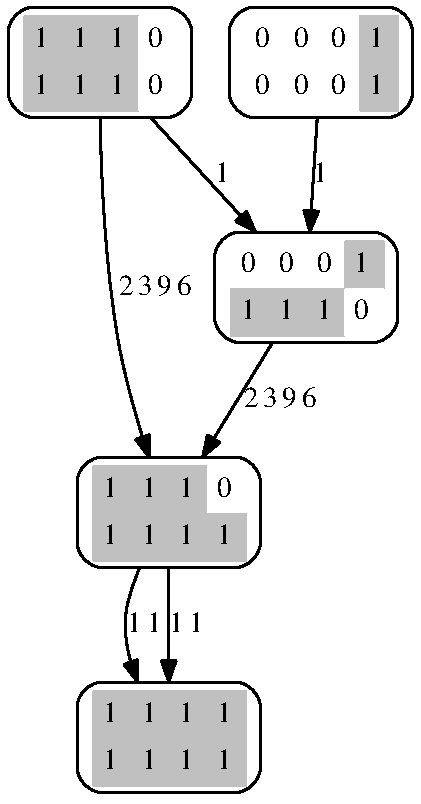
\includegraphics[scale=.35]{images/pepper_3_3}
  }
  \hspace{1cm}
  \subfloat[${F=4}$, ${G=4}$, ${\mathrm{pop} = 633}$ and ${\mathrm{obj} = 7.13}$]{\label{fig:pepper_4_4}
    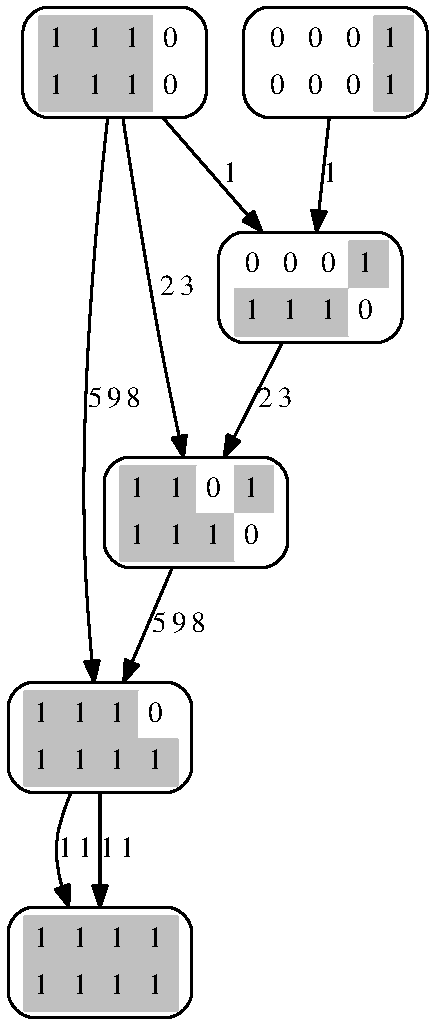
\includegraphics[scale=.35]{images/pepper_4_4}
  }
  \caption{Crossing schedules for the pepper instance. Inner nodes are obtained via crossings requiring a population size shown on the arcs, in both schedules the final crossing is a selfing. Chromosomes of an inner node are obtained via crossovers in their parents. Schedule (b) is provably optimal.}
  %\caption{Crossing schedules for the pepper instance, (b) is provably optimal.}
  \label{fig:pepper}
\end{figure}

\subsubsection{Generated instances.} Due to the lack of further real-world instances, we generate random instances on which we evaluate the performance of our method. The generated instances either have 5 or 10 parents and concern 4 up to 8 loci. The number of correct alleles per parental genotype affects the difficulty of the instances, we vary this number depending on the number of loci. In total 140 instances are generated, among which 20 concern instances of 4 loci; the classes of 5-8 loci are comprised by 30 instances each. We run both the DAG and the tree version of the MIP on all instances. For the DAG case, we were able to obtain solutions to 128 instances compared to 119 instances (see Figure~\ref{fig:tree}) for the tree version. Among the unsolved instances for the tree case, there are also instances that are infeasible due to the value of $N_\mathrm{max}$ which requires re-use of genotypes. The number of instances that were solved to provable optimality in the DAG case is 58; for the tree case this number is 89. According to Figure~\ref{fig:ratio}, DAGs provide a gain in solution quality of up to 5\% on average compared to the tree. Note that none of the instances is of the nature that is captured by Servin's model. Not surprisingly, trees are easier to solve as can be seen in Figure~\ref{fig:runningtimes}.

\begin{figure}
  \center
  \subfloat[Optimality of solutions]{\label{fig:dag}\label{fig:tree}
    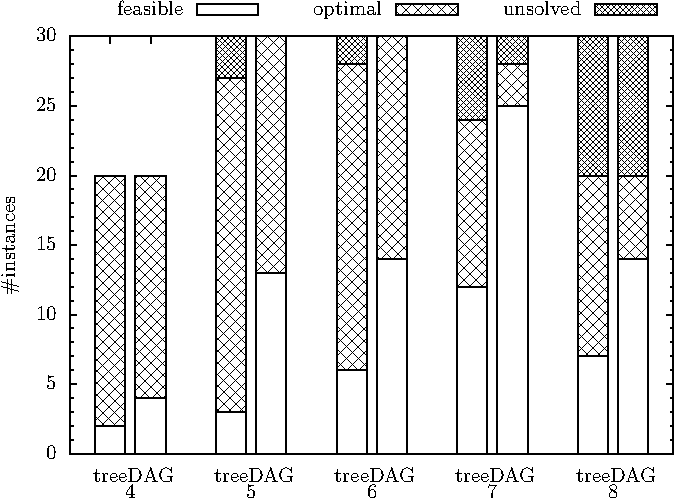
\includegraphics[scale=0.5]{images/plot_optimality}
  }
  \hspace{.25cm}
  \subfloat[Running times (instances exceeding the time limit were not considered), objective value ratio (right y-axis)]{\label{fig:runningtimes}\label{fig:ratio}
    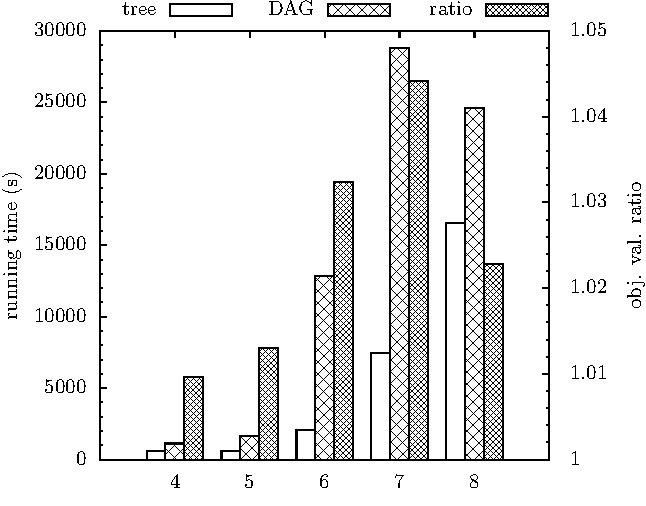
\includegraphics[scale=0.5]{images/plot_time_ratio}
  }
  \caption{Results for generated instances}
  \label{fig:performance}
\end{figure}

\section{Conclusion}
\label{sec:discussion}

For the first time we have described a mathematical model capturing the problem of marker-assisted gene pyramiding to its full extent. We show that our approach is capable of solving a real-world instance and generated instances, often to provable optimality.
As mentioned earlier, our method is not exact due to (i) the piecewise-linear approximation of the population size function and (ii) a simplification in \eqref{eq:something} of neglecting the possibility that the two chromosomes may swap their originating genotypes. However, in our experiments we have not observed any crossing where this could have happened. 
The NP-hardness proof involves only the number of crossings; as for the number of generations, the same reduction can be applied. The hardness with respect to the population size remains open. Possible extensions to our problem definition include considering heterozygous ideotypes. This requires an extension to tertiary alleles. Another extension would be to consider so called `don't care' alleles, which are alleles that are not preserved due to crossover events, and as such do not need to be considered in the probability function.

\subsubsection{Acknowledgments.} We would like to thank Bertrand Servin for kindly providing us the source code of his method. In addition we are very grateful for the constructive comments of the anonymous referees.

\bibliographystyle{abbrv}
\bibliography{cso}

\appendix
 
%\subsection{Lemma~\ref{lem:selfing}}

\section{Complete MIP}
\label{sec:complete_mip}

Given $(F, G)$ as the number of crossings and the number of generations, respectively, and $L = F + n$, the MIP is as follows.

\begingroup
\allowdisplaybreaks
\begin{align*}
\min\quad        & \sum_{i=n+1}^L\sum_{j=1}^{\ell+1} \lambda^i_j\cdot N(\mathrm e^{a_j},\gamma) & \label{CS} \tag{CSO}\\
\text{s.t.}\quad & \sum_{j=1}^{\delta(k)- 1} x_{k,j}                                  && =     1              && {\scriptstyle 2n < k \leq 2L}\\
                 & g_{k,p,2i}   - a_{2i,p}   \cdot x_{k,i} \cdot (1-y_{k,p})          && =     0              && {\scriptstyle 2n < k \leq 2L, 1 \leq p \leq m, 1 \leq i < \delta(k)}\\
                 & g_{k,p,2i-1} - a_{2i-1,p} \cdot x_{k,i} \cdot y_{k,p}              && =     0              && {\scriptstyle 2n < k \leq 2L, 1 \leq p \leq m, 1 \leq i < \delta(k)}\\
                 & \sum_{i = 1}^{\delta(k) - 1} (g_{k,p,2i-1} + g_{k,p,2i})           && = a_{k,p}            && {\scriptstyle 2n < k \leq 2L, 1 \leq p \leq m}\\
                 & a_{2i-1,p}                                                         && = c^i_{1,p}          && {\scriptstyle 1 \leq i \leq n, 1 \leq p \leq m}\\
                 & a_{2i,p}                                                           && = c^i_{2,p}          && {\scriptstyle 1 \leq i \leq n, 1 \leq p \leq m}\\
                 & a_{2L-1,p}                                                         && = c^*_{1,p}          && {\scriptstyle 1 \leq p \leq m}\\
                 & a_{2L,p}                                                           && = c^*_{2,p}          && {\scriptstyle 1 \leq p \leq m}\\
                 & |a_{2i-1,p} - a_{2i,p}|                                            && = \tilde{a}_{i,p}    && {\scriptstyle 1 \leq i \leq L, 1 \leq p \leq m}\\
                 & h_i                                                                && \geq \tilde{a}_{i,p} && {\scriptstyle 1 \leq i \leq L, 1 \leq p \leq m}\\
                 & \sum_{r=p+1}^q |y_{k,r} - y_{k,r-1}|                               && = z_{k,p,q}          && {\scriptstyle 2n < k \leq 2L,\, 2 \leq p < q \leq m}\\
                 & \tilde{a}_{i,p}\cdot\tilde{a}_{i,q}\cdot\prod_{r=p+1}^{q-1}(1-\tilde{a}_{i,r}) &&  = b_{i,p,q} && {\scriptstyle 1 \leq i \leq L, 1 \leq p<q \leq m}\\
                 & \sum^{i-1}_{j=1}\sum_{k=2i-1}^{2i}x_{k,j}\bigg(h_j\ln(\frac{1}{2})\\
                 & \quad + \sum_{p=1}^{m-1}\sum_{q=p+1}^m b_{j,p,q}\ln(1-r_{p,q})\\
                 & \quad + \sum_{p=1}^{m-1}\sum_{q=p+1}^m  b_{j,p,q} \cdot z_{k,p,q} \ln(\frac{r_{p,q}}{1-r_{p,q}}) \bigg) && = \bar{z}_i && {\scriptstyle n < i \leq L}\\
                 & \sum_{j=1}^{\ell+1} \lambda^i_j                                    && = 1                  && {\scriptstyle n < i \leq L}\\
                 & \sum_{j=1}^{\ell+1} \lambda^i_j\cdot d_j                           && = \bar{z}_i          && {\scriptstyle n < i \leq L}\\
                 & \lambda^i_j                                                        && \geq 0               && {\scriptstyle n < i \leq L, 1 \leq j \leq \ell+1}\\
                 & |x_{2i-1,j} - x_{2i,j}|                                            && \leq h_j             && {\scriptstyle n < i \leq L, 1 \leq j < i}\\
                 & x_{k,j}                                                            && \in \{0,1\}          && {\scriptstyle 2n < k \leq 2L, 1 \leq i < \delta(k)}\\
                 & g_{k,p,l}                                                          && \in \{0,1\}          && {\scriptstyle 2n < k \leq 2L, 1 \leq p \leq m, 1 \leq l<2\delta(k)-1}\\
                 & a_{k,p}                                                            && \in \{0,1\}          && {\scriptstyle 1 \leq k \leq 2L, 1 \leq p \leq m}\\
                 & y_{k,p}                                                            && \in \{0,1\}          && {\scriptstyle 2n < k \leq 2L, 1 \leq p \leq m}\\
                 & \tilde{a}_{i,p}                                                    && \in \{0,1\}          && {\scriptstyle 1 \leq i \leq L, 1 \leq p \leq m}\\
                 & h_{i}                                                              && \in \{0,1\}          && {\scriptstyle 1 \leq i \leq L}\\
                 & b_{i,p,q}                                                          && \in \{0,1\}          && {\scriptstyle 1 \leq i \leq L, 1 \leq p<q \leq m}\\
                 & z_{k,p,q}                                                          && \in \mathbb{N}       && {\scriptstyle 2n < k \leq 2L,\, 2 \leq p < q \leq m}\\
                 & \bar{z}_{i}                                                        && \in \mathbb{R}       && {\scriptstyle n < i \leq L}\\
                 & \lambda^i_j                                                        && \in \mathbb{R}       && {\scriptstyle n < i \leq L, 1 \leq j \leq \ell+1}
\end{align*}
\endgroup

\begin{align*}
{\scriptstyle\min\;}& {\scriptstyle\alpha\cdot\sum_{j=2}^{k}  c_j \sum_{i=1}^{2L} z_{i,j} + \beta\cdot\sum_{i-1}^L v_i +\gamma\cdot d }&\label{CS} \tag{CSO}\\
{\scriptstyle \text{s.t.}\;   \sum_{j=1}^{i-1} e_{2i-1,j} }&{\scriptstyle \leq 1 }&&{\scriptstyle 1\leq i\leq L} \\
{\scriptstyle        \sum_{j=1}^{i-1} x_{2i-1,j}- \sum_{j=1}^{i-1} e_{2i,j}}&{\scriptstyle=0 }&&{\scriptstyle1\leq i\leq L} \\
 {\scriptstyle      g_{i,t,2j} }&{\scriptstyle\leq x_{i,j} }&&{\scriptstyle 3\leq i \leq 2L, 1\leq t \leq k, 1\leq j\leq\lfloor\frac{i-1}{2} \rfloor}  \\
 {\scriptstyle      g_{i,t,2j-1} }&{\scriptstyle\leq x_{i,j} }&&{\scriptstyle 3\leq i \leq 2L, 1\leq t \leq k, 1\leq j\leq\lfloor\frac{i-1}{2} \rfloor } \\
 {\scriptstyle      g_{i,t,j} }&{\scriptstyle\leq b_{j,t}} &&{\scriptstyle 3\leq i \leq 2L, 1\leq t \leq k, 1\leq j\leq i-2+(i\mod 2)} \\
 {\scriptstyle      g_{i,t,j} }&{\scriptstyle\leq 1-y_{i,t} }&&{\scriptstyle 3\leq i \leq 2L, 1\leq t \leq k, 1\leq j<i, j \mbox{ \scriptsize  odd}}\\
 {\scriptstyle      g_{i,t,j} }&{\scriptstyle\leq y_{i,t} }&&{\scriptstyle 3\leq i \leq 2L, 1\leq t \leq k, 1\leq j<i, j \mbox{ \scriptsize even}}\\
 {\scriptstyle      g_{i,t,2j-1} }&{\scriptstyle\geq e_{i,j} +  b_{2j-1,t} + 1-y_{i,t} -2 }&&{\scriptstyle 3\leq i \leq 2L, 1\leq t \leq k, 1\leq j\leq\lfloor\frac{i-1}{2} \rfloor} \\
 {\scriptstyle      g_{i,t,2j} }&{\scriptstyle\geq e_{i,j} +  b_{2j,t} + y_{i,t} -2 }&&{\scriptstyle 3\leq i \leq 2L, 1\leq t \leq k, 1\leq j\leq\lfloor\frac{i-1}{2} \rfloor} \\
  {\scriptstyle     g_{i,t,2j} }&{\scriptstyle\leq l_{2j,t}\cdot e_{i,j} }&&{\scriptstyle 1\leq i \leq 2L, 1\leq t \leq k, 1\leq j\leq m}\\
  {\scriptstyle     g_{i,t,2j-1} }&{\scriptstyle\leq l_{2j-1,t}\cdot e_{i,j} }&&{\scriptstyle 1\leq i \leq 2L, 1\leq t \leq k, 1\leq j\leq m}\\
   {\scriptstyle    g_{i,t,2j} }&{\scriptstyle\leq l_{2j,t}\cdot y_{i,t} }&&{\scriptstyle 1\leq i \leq 2L, 1\leq t \leq k, 1\leq j\leq m}\\
  {\scriptstyle     g_{i,t,2j-1} }&{\scriptstyle\leq l_{2j-1,t}\cdot (1-y_{i,t}) }&&{\scriptstyle 1\leq i \leq 2L, 1\leq t \leq k, 1\leq j\leq m}\\
  {\scriptstyle     g_{i,t,2j} }&{\scriptstyle\geq l_{2j,t}\cdot(e_{i,j}+ y_{i,t}-1) }&&{\scriptstyle 1\leq i \leq 2L, 1\leq t \leq k, 1\leq j\leq m} \\
  {\scriptstyle     g_{i,t,2j-1} }&{\scriptstyle\geq l_{2j-1,t}\cdot(e_{i,j}+ (1-y_{i,t})-1) }&&{\scriptstyle 1\leq i \leq 2L, 1\leq t \leq k, 1\leq j\leq m} \\
  {\scriptstyle     \sum_{j=1}^{i-2+(i\mod 2)} g_{i,t,j} - b_{i,t} }&{\scriptstyle=0 }&&{\scriptstyle 1\leq i \leq 2L, 1\leq t \leq k}\\
  {\scriptstyle z_{i,t} }&{\scriptstyle\geq y_{i,t}-y_{i,t-1}}&&{\scriptstyle 1\leq i \leq 2L, 2\leq t \leq k}\\
  {\scriptstyle z_{i,t} }&{\scriptstyle\geq y_{i,t-1}-y_{i,t}}&&{\scriptstyle 1\leq i \leq 2L, 2\leq t \leq k}\\
  {\scriptstyle      v_i-\sum_{j=1}^{i-1} e_{2i-1,j}}&{\scriptstyle=0}&&{\scriptstyle1\leq i \leq L}\\
   {\scriptstyle    t_i}&{\scriptstyle \leq v_i}&&{\scriptstyle 1\leq i \leq L}\\
     {\scriptstyle     t_i}&{\scriptstyle \leq 1-b_{2i-1,t} }&&{\scriptstyle 1\leq i \leq L,1\leq t \leq k: \mbox{ \scriptsize target}_1(t)=0}\\  
     {\scriptstyle     t_i}&{\scriptstyle \leq b_{2i-1,t} }&&{\scriptstyle 1\leq i \leq L,1\leq t \leq k: \mbox{ \scriptsize target}_1(t)=1}\\  
     {\scriptstyle     t_i}&{\scriptstyle \leq 1-b_{2i,t} }&&{\scriptstyle 1\leq i \leq L,1\leq t \leq k: \mbox{ \scriptsize  target}_2(t)=0}\\  
     {\scriptstyle     t_i}&{\scriptstyle \leq b_{2i,t} }&&{\scriptstyle 1\leq i \leq L,1\leq t \leq k: \mbox{ \scriptsize target}_2(t)=1}\\  
     {\scriptstyle     \sum_{i=1}^L t_i }&{\scriptstyle=1 }&& \\
   {\scriptstyle r_i }&{\scriptstyle \geq r_j+1 - L\cdot (2-e_{2i-1,m+j}-v_j)} &&{\scriptstyle 1\leq i\leq L, 1\leq j \leq i}\\
   {\scriptstyle r_i }&{\scriptstyle \geq r_j+1 - L\cdot (2-e_{2i,m+j}-v_j) }&&{\scriptstyle 1\leq i\leq L, 1\leq j \leq i}\\
    {\scriptstyle      r_i }&{\scriptstyle \geq 1 }&&{\scriptstyle 1\leq i \leq L}\\
   {\scriptstyle d }&{\scriptstyle \geq r_i }&&{\scriptstyle 1\leq i \leq L}\\
   {\scriptstyle b_{i,t}, y_{i,t}, v_{i'}, g_{i,t,j}  }&{\scriptstyle \in \{0,1\}} &&{\scriptstyle 1\leq i\leq 2L, 1\leq t \leq k, 1\leq i'\leq L \notag}\\
   {\scriptstyle e_{i,j}}& {\scriptstyle \in \{0,1\}}&&{\scriptstyle 1\leq i\leq 2L, 1\leq j\leq m+\lfloor\frac{i-1}{2} \rfloor }\notag\\
   {\scriptstyle z_{i,t} }&{\scriptstyle \in \{0,1\} }&&{\scriptstyle 1\leq i\leq 2L, 2\leq t \leq k}\notag\\
{\scriptstyle r_i, d }&\; \text{integer.}&& \notag
\end{align*}

\end{document}
